\subsubsubsubsection{UEDirector}
\begin{figure}[h]
\centering
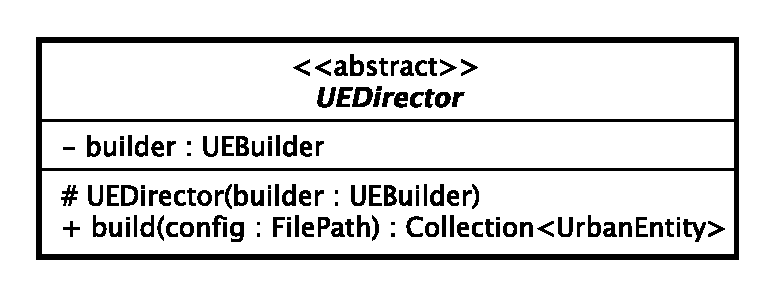
\includegraphics[scale=0.6,keepaspectratio]{images/solution/u_e_director.eps}
\caption{\pReactiveBuild::UEDirector}
\label{fig:sd-app-uedirector}
\end{figure}
\FloatBarrier
\begin{itemize}
  \item \textbf{\descr} \\
    It represents the urban entity director which instructs the builder.
  \item \textbf{\attrs}
  \begin{itemize}
    \item \texttt{builder: UEBuilder} \\
The builder object which builds parts of the district.
  \end{itemize}
  \item \textbf{\ops}
  \begin{itemize} 
    \item[\#] \texttt{UEDirector(builder: UEBuilder)} \\
Creates a director with its own builder object.
    \item[+] \texttt{build(config: FilePath) : Collection<UrbanEntity>} \\
Builds a collection of urban entities according to the configuration file. It uses the
builder multiple times to create incrementally a configuration of the requested
urban entity as specified in the configuration file.
  \end{itemize}
\end{itemize}
